\section{Dataset and Experiment Design} \label{design}
In this section, we introduce the dataset \textit{CORe50} realeased by CVPR Workshop. Their dataset consist of three parts, and due to the constraint of time, we only consider the first two part of the three challenges. Then, we select two representative approaches for Continual Learning, EWC and Piggyback, and introduce the theorem and some core details about them.

\subsection{Dataset and Tasks}
\textit{CORe50} is a new dataset specially designed for \textit{(C)ontinual (O)bject (Re)cognition}. Unlike \textit{permuted MNIST}  where new tasks to learn are obtained by simply scrambling the pixel positions, \textit{CORe50} is much more complex and a real life dataset. Datasets such as \textit{ImageNet} and \textit{Pascal VOC} provide a good playground for image classification and detection, but they have been designed with “static” evaluation and lack of multiple views of the same objects taken into different sessions, \textit{CORe50} solves the above problems and meets the requirement for continuous learning scenarios on computer vision.

It consists 50 domestic objects belonging to 10 categories. The dataset is separated into 11 distinct sessions (8 indoors and 3 outdoors) with different background and lightning. For each session and for each object, a 15 seconds video (at 20 fps) has been recorded with a Kinect 2.0 sensor delivering 300 RGB-D frames. The whole dataset consists of 164,866 128 × 128 RGB-D images: 11 sessions x 50 objects x (∼300*) frames per session.  Three of the eleven sessions (\#3, \#7 and \#10) have been selected for test and the remaining 8 sessions are used for training. 

\begin{figure}[h]
  \centering
  \captionsetup{width=0.6\textwidth}
  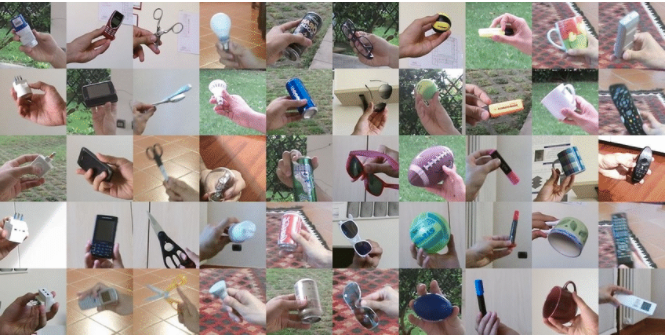
\includegraphics[width=0.8\textwidth]{figure/core50.png}
  \caption{Example images of the 50 objects in CORe50. Each column denotes one of the 10 categories.}
  \label{core50}
\end{figure}

There are three tasks in CVPR 2020 Workshop \textit{CLVision Challenge}:
\begin{itemize}
\item \textbf{New Classes(NC)}: New training patterns belonging to different classes become available in subsequent batches. In this case the model should be able to deal with the new classes without losing accuracy on the previous ones.
\item \textbf{New Instances(NI)}: New training patterns of the same classes become available in subse- quent batches with new poses and conditions (illumination, background, occlusion, etc.). A good model is expected to incrementally consolidate its knowledge about the known classes without compromising what it has learned before.
\item \textbf{New Instances and Classes(NIC)}: New training patterns belonging both to known and new classes become available in subsequent training batches. A good model is expected to consolidate its knowledge about the known classes and to learn the new ones.
\end{itemize} 

\subsection{EWC}
In brains, synaptic consolidation enables continual learning by reducing the plasticity of synapses that are vital to previously learned tasks.  \textit{EWC} is an algorithm that performs a similar operation in artificial neural networks by constraining important parameters to stay close to their old values. \textit{EWC} can be used in supervised learning and reinforcement learning problems to train several tasks sequentially without forgetting older ones.

\begin{figure}[h]
  \centering
  \captionsetup{width=0.6\textwidth}
  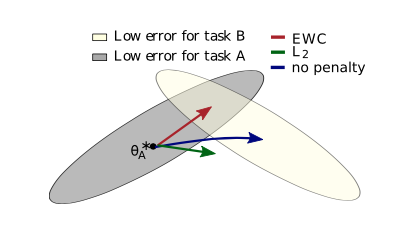
\includegraphics[width=0.8\textwidth]{figure/ewc.png}
  \caption{By applying \textit{EWC}, the model of the weights can learn the new task while still maintain in the range of solving the old task. (Red arrow)}
  \label{EWC}
\end{figure}

\subsubsection{Theorem}
From a probabilistic perspective: optimizing the parameters is tantamount to finding their most probable values given some data D. We can compute this conditional probability $p(\theta | \mathcal{D})$ from the prior probability of the parameters $p(\theta)$ and the probability of the data $p(\mathcal{D}|\theta)$ by using Bayes’ rule:

\begin{equation}
\begin{aligned}
\log p(\theta | \mathcal{D})=\log p\left(\mathcal{D}_{B} | \theta\right)+\log p\left(\theta | \mathcal{D}_{A}\right)-\log p\left(\mathcal{D}_{B}\right)
\end{aligned}
\end{equation}

Similarly we can apply Bayes' rule on two continuous tasks A and B: 

\begin{equation}
\begin{aligned}
\log p(\theta | \mathcal{D})=\log p\left(\mathcal{D}_{B} | \theta\right)+\log p\left(\theta | \mathcal{D}_{A}\right)-\log p\left(\mathcal{D}_{B}\right)
\end{aligned}
\end{equation}

While $\log p(\mathcal{D}_{B}|\theta)$ is negative training loss for task B, we can optimize this by gradient descent.
$\log p(\mathcal{D}_{B})$ is a constant, we don't need to care about it when optimizing for the overall goal. $\log p(\theta|\mathcal{D}_{A})$ ‘s real value is intractable and will be approximated by Laplace approximation. The approximated value can further be the derivation regarding approximated mean value and its corresponding Hessian matrix. Noted that the expected value of Hessian matrix is the negative value of Fisher information matrix $F$, thus the original goal of maximizing $\log p(\theta | \mathcal{D})$ is equivalent to minimizing the following loss function:

\begin{equation}
\mathcal{L}(\theta)=\mathcal{L}_{B}(\theta)+\sum_{i} \frac{\lambda}{2} F_{i}\left(\theta_{i}-\theta_{A, i}^{*}\right)^{2}
\end{equation}

where $\mathcal{L}_{\mathcal{B}}(\theta)$ is the loss for task B only and hyperparameter $\lambda$ sets how important the old task is compared to the new task. When the third task comes, you can treat all previous tasks as the old task and repeat the above process. In the end, it can ensure the model can learn new tasks without changing the weights for the previous tasks too much. 

\subsubsection{Experiment Setting}
After several experiments, we set the hyperparameter $\lambda$ = 100, which we think it is an appropriate value of how important the old task is to the new task. The best results are produced by SGD as the optimizer.




\subsection{Piggyback}
Piggyback is a upgrading version of Packnet, it uses pure mask layer to mask weights for new task. In this part, we introduce the core idea and the mathemetical representation of Piggyback. We also demonstrate some of the techniques used in training for Piggyback.

\subsubsection{Theorem}
\begin{figure}[h]
  \centering
  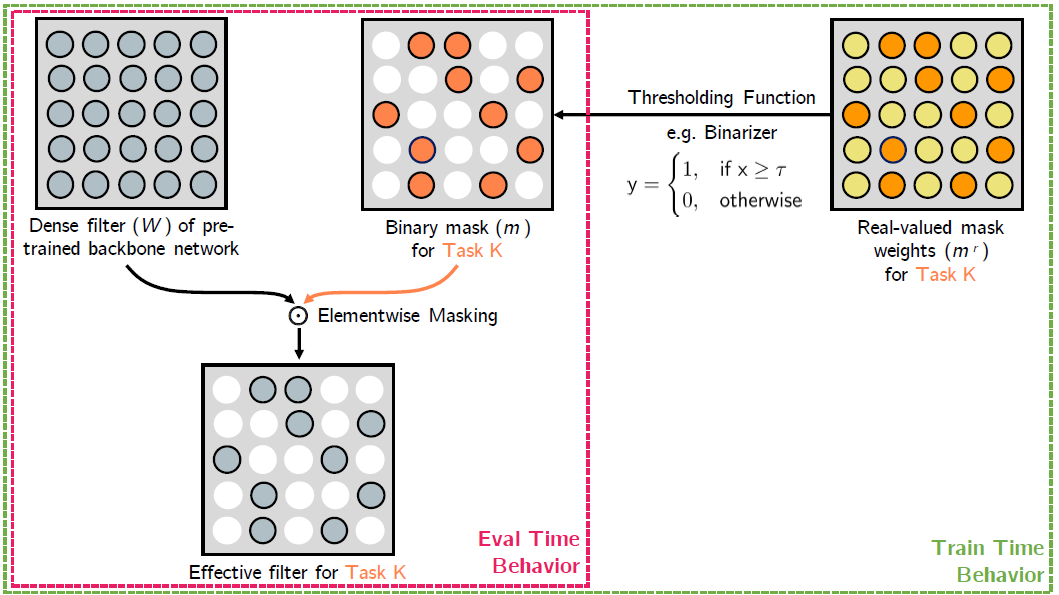
\includegraphics[width=0.8\textwidth]{figure/piggyback.png}
  \caption{Piggyback Overview}
  \label{piggy}
\end{figure}

Piggyback adopts masking weight for new task to overcome catastrophic forgetting. The core idea is to selectively mask the fixed weights of a base network, and then use this mask to predict the new task. That is, given model $\mathbf{W}$, whenever there is a new task streaming in, the model will initialize and optimize a binary value matrix $\mathbf{m}$, and use this mask to generate weight $\mathbf{W^\star}$ to be used in prediction for this specific new task. The gradient that backpropagates to the layer will not affect $\mathbf{W}$ but $\mathbf{m}$. In this way, for a given task, we can obtain filters that is consist of 0/1. For example, a dense weight vector [0.1, 0.2, 0.3, 0.4] could be filtered to [0, 0.2, 0.3, 0] after the binary masking. In short, we does not learn what are the `right` parameters but learn what is not the `right` parameters. Therefore, the choice of backbone network is crucial to the performance of piggyback because if the original weights are malfunctioning, pure masking cannot greatly improve the accuracy.

The structure of \textit{Piggyback} is shown in Figure \ref{piggy}. To explain the procedure for training, we consider an end to end fully-connected layer case. Denote $\mathbf{x}=[x_1, x_2, ..., x_m]$ as input, and $\mathbf{y}=[y_1, y_2, ..., y_n]$ as output. The weight matrix for this layer is $\mathbf{W}^{n\times m}$. Without loss of genrality, we can simply assume $\mathbf{y}=\mathbf{W}\mathbf{x}$ by ignoring the bias term. Suppose the loss function is $L$, the normal backpropagation equation for $\mathbf{W}$ is,
\begin{equation}
\centering
\begin{aligned}
\delta w_{ji}&=\frac{\partial L}{\partial w_{ji}} = (\frac{\partial L}{\partial y_j})\cdot (\frac{\partial y_j}{\partial w_{ji}}) \\
&= \delta y_j \cdot x_j \\
\therefore \delta \mathbf{W} &= \delta \mathbf{y} \cdot  \mathbf{x^T} \\
\end{aligned}
\end{equation}
In \textit{Piggyback}, the author has introduced a real value mask matrix $\mathbf{M_r}^{n\times m}$ and a manually set threshold $\tau$. $M_r$ is used to create the binary mask matrix $\mathbf{M}=[m_{ji}]$. We can obtain $m_{ji}$ by,
\begin{equation}
m_{ji}=\begin{cases}
1,\ \ &{\rm if}\ m^r_{ji}>\tau \\
0,\ \ &{\rm otherwise} \\
\end{cases}
\end{equation}
Then, for $y_j\in\mathbf{y}$, it gives $y_j=\sum_{i=1}^m w_{ji}\cdot m_{ji} \cdot x_i$. The backpropagation equation is used to update the real value matrix $M_r$. That is, during the whole training procedure, the weight matrix $\mathbf{W}$ is fixed as constant. In \textit{Piggyback}, the modified mask weigths updates as follows. Here, $A\odot B = C=[c_{ji}=A_{ji}B_{ji}]$. 

\begin{equation}
\begin{aligned}
\delta m_{ji}=\frac{\partial L}{\partial m_{ji}} &= (\frac{\partial L}{\partial y_j})\cdot (\frac{\partial y_j}{\partial m_{ji}}) \\
&= \delta y_j \cdot w_{ji} \cdot x_j \\
\therefore \delta \mathbf{m} &= (\delta \mathbf{y} \cdot x^T) \odot \mathbf{W} \\
\end{aligned}
\end{equation}
\subsubsection{Experiment Setting}
In practical, it is hard to derive the analytical solution to threshold $\tau$. In the original work, the author set $\tau=5e-3$. As for the matrix $\mathbf{m_r}$, the author initialized the value to 0.01. The best results are produced by Adam optimizer. In our experiment, we have inherited the parameter settings in the work. However, as mentioned in the previous statement, the crucial part for \textit{Piggyback} is that the base model have to be fine-tuned, otherwise the model will not work very well. We have also verified such phenomon in our experiment. To improve the performance, we modified the logic of the model. At the first task, we use the pure base model to perform the training, as the pre-trained network(ResNet50\cite{he2016deep}, in our case)cannot perform well on the given dataset. Then we begin performing mask and \textit{Piggyback}. This part will later be discussed in detail in Section \ref{eval}.





